
The United States have been the forerunner of nuclear energy, with a current
installed capacity of about 100 GWe. With its size and long history of nuclear
energy, the United States have accumulated about $70,000$ \gls{MTHM} of \gls{UNF}.

The problem with modeling the U.S. transition scenario is that the U.S. does not have
a defined advanced reactor, whereas France has a central plan to transition into \glspl{ASTRID} \cite{boullis_french_2015, varaine_pre-conceptual_2012}.
Although the most prominent and `canonical' reactor design when considering
transition into fast-spectrum, breeding reactors ]is the \gls{SFR},
the fact that the U.S. nuclear reactor fleet
is decided by economic interests (industries), this allows me to explore
different options, such as the \gls{MSR} design.

\glspl{MSR} reactor designs have recently gained attention in the U.S. due to it being a
potentially safer, more efficient, and sustainable form of nuclear power
\cite{serp_molten_2014}. Multiple companies in the U.S. are now pursuing
commercialization of \gls{MSR} design reactors, such as Tranasatomic \cite{transatomic_power_corporation_technical_2016}
, Terrapower, Terrestrial \cite{leblanc_18_2017}, and
Thorcon \cite{jorgensen_19_2017}. Other parties such as China (TMSR-LF \cite{dai_17_2017}) 
and the European Union (MSFR \cite{heuer_towards_2014}, MOSART \cite{ignatiev_molten_2014})
are developing \gls{MSR} designs.

In this chapter, I explore the U.S. transition scenario
from a \gls{LWR} fleet into a \gls{MSR} fleet.

\section{Initial Conditions and Scenario Parameters}
Unlike the French scenario,
where the \gls{UNF} inventory at the present time is calculated by
simulating the nuclear operational history from 1970, there is a
detailed database that describes the U.S. \gls{UNF} inventory up to May of 2013.
The \gls{UNF-STANDARDS} database is a comprehensive,
controlled source of \gls{UNF} information, including dry cask attributes, assembly
data, and economic attributes \cite{peterson_unf-st&dards_2017}. This database
allows the transition scenario simulation to start from 2013, instead of 1970,
as in the French simulation. The \gls{UNF} inventory mass and composition in 2013
will be imported from \gls{UNF-STANDARDS} and will be `initiated' in the simulation
as a \texttt{Source} facility. The total mass of \gls{UNF} listed
in the \gls{UNF-STANDARDS} database is 68,072 MTHM.

The U.S. nuclear fleet in 2013 can be extracted from the \gls{PRIS} database.
The same assumption that legacy reactors have a 60-year lifetime is applied.
I used \texttt{write\_input.py} to generate the expected power capacity
of the current U.S. nuclear from 2013 (shown in figure \ref{fig:us_legacy}).

\begin{figure}[htbp!]
	\begin{center}
		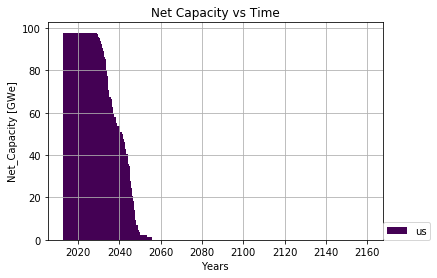
\includegraphics[scale=0.6]{./images/us/legacy_power.png}
	\end{center}
	\caption{Installed nuclear capacity in the United States from 2013.}
	\label{fig:us_legacy}
\end{figure}

The U.S. had 101 reactor units operating in 2013. Two reactors -
Vermont Yankee and Fort Calhoun one - has shut down since 2013.
Vermont Yankee was shut down in December, 2014, and Fort
Calhoun one was shut down in October, 2016. At the date of this
work, the United States has 99 commercial reactors with a 
net capacity of 100,350 \gls{MWe} \cite{iaea_nuclear_2017}.

\subsection{Energy Demand Prediction}
The reference for the energy demand prediction is the 
\gls{EIA} Annual Energy Outlook.
The 2018 Annual Energy Outlook report predicts an annual electricity demand growth
of 0.9\% \cite{u.s._annual_2018}. The report also predicts that nuclear
energy will either remain static or decrease. However, for this work,
I assume that the U.S. nuclear energy capacity increases at an annual
rate of 0.9\% from 2020 (shown in figure \ref{fig:us_proj}).

\begin{figure}[htbp!]
	\begin{center}
		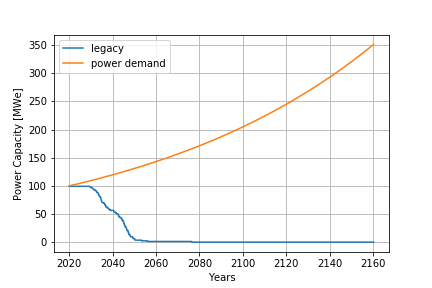
\includegraphics[scale=0.6]{./images/us/projection.png}
	\end{center}
	\caption{Projected nuclear power demand from 2020, with an
			 annual increase rate of 0.9\%.}
	\label{fig:us_proj}
\end{figure}

\section{U.S. Deployment Schedule}

\section{Scenario Specification}

\section{Reactor Specifications}

\section{Material Definitions}

\section{Results}

\section{Conclusion}